\begin{enumerate}
	\item Exercício
	
	\begin{equation*}
		f(x,y) = x^3;\; 0 \leq x \leq 2;\; x^2 \leq y \leq 4	
	\end{equation*}
	\begin{equation*}
		\iint_R f(x, y) dy dx
	\end{equation*}
	
	\begin{figure}[htb]
		\caption{Integrais duplas - Aula 5 - Exercício I}
		\label{v05_a05_e01}
		\centering
		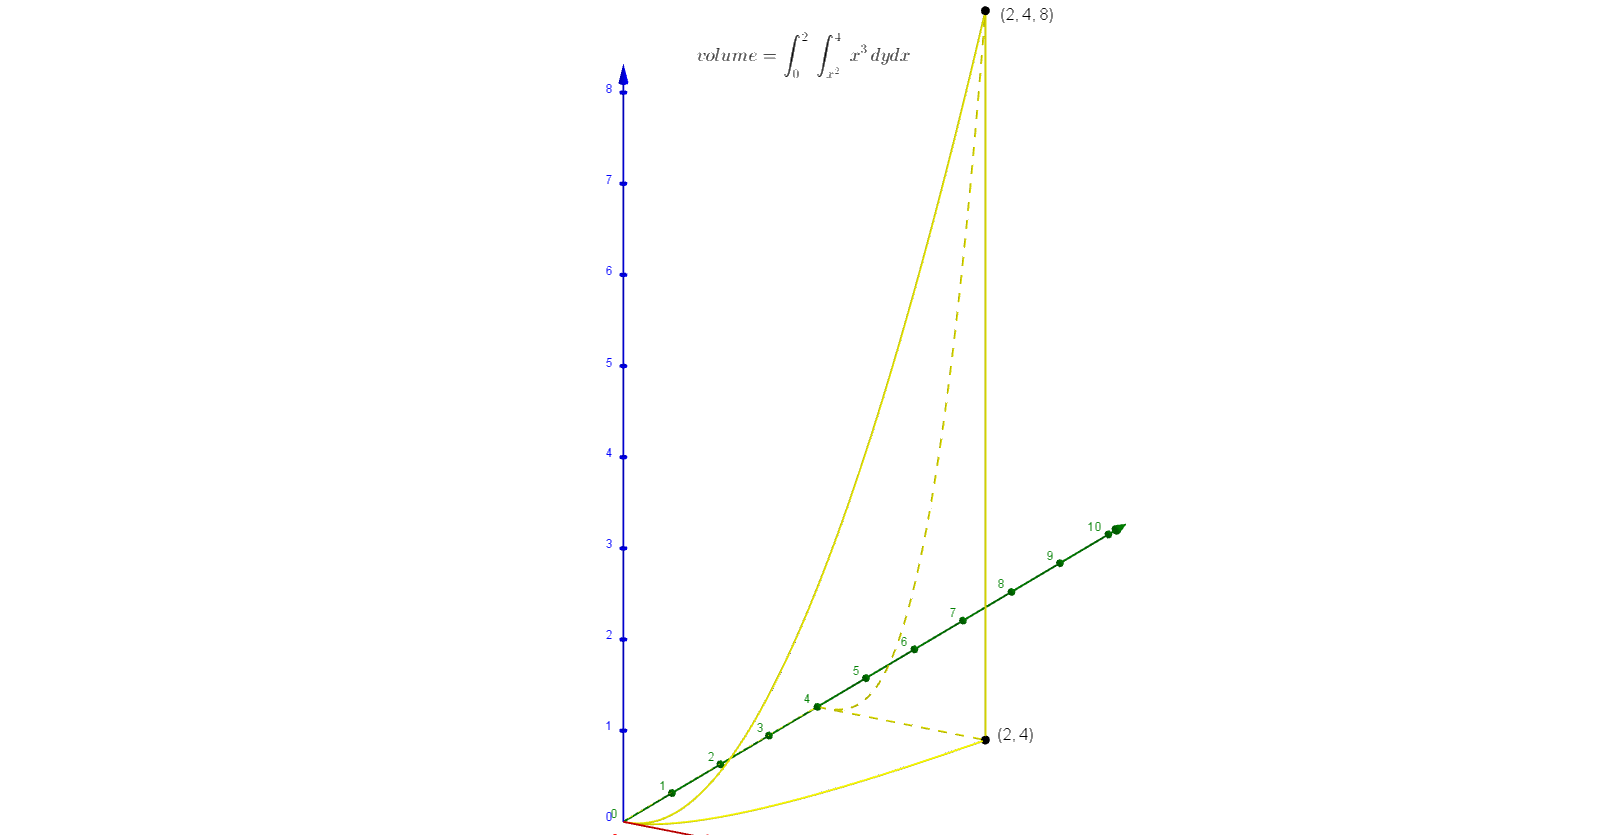
\includegraphics[width=0.5\textwidth]{v05_a05_e01.png}		
	\end{figure}
	
	\begin{gather*}
		v = \int_0^2 \int_{x^2}^4 x^3\, dy dx = \int_0^2 x^3\, dx \int_{x^2}^4 dy = \int_0^2 x^3\, dx\, [y]_{x^2}^4 = \int_0^2 x^3\, dx\, \left[4 - x^2\right] =\\ 4\int_0^2 x^3\, dx - \int_0^2 x^5\, dx = \left[\overstrike{4}\dfrac{x^4}{\overstrike{4}} - \frac{x^6}{6}\right]_0^2 = \left[\dfrac{6x^4 - x^6}{6}\right]_0^2 = \frac{1}{6}\left[x^4\left(6 - x^2\right)\right]_0^2 =\\ \frac{1}{6}\left[2^4\left(6 - 2^2\right) - \overstrike{0^4\left(6 - 0^2\right)}\right] = \dfrac{1}{6}(16\cdot2) = \dfrac{32}{6} = \dfrac{16}{3} = 5,2
	\end{gather*}
	
	\item Exercício
	
	\begin{equation*}
		f(x,y) = x^2y;\; 1 \leq x \leq 3;\; x \leq y \leq 2x + 1
	\end{equation*}
	\begin{equation*}
		\iint_R f(x, y) dy dx
	\end{equation*}
	
	\begin{figure}[htb]
		\caption{Integrais duplas - Aula 5 - Exercício II}
		\label{v05_a05_e02}
		\centering
		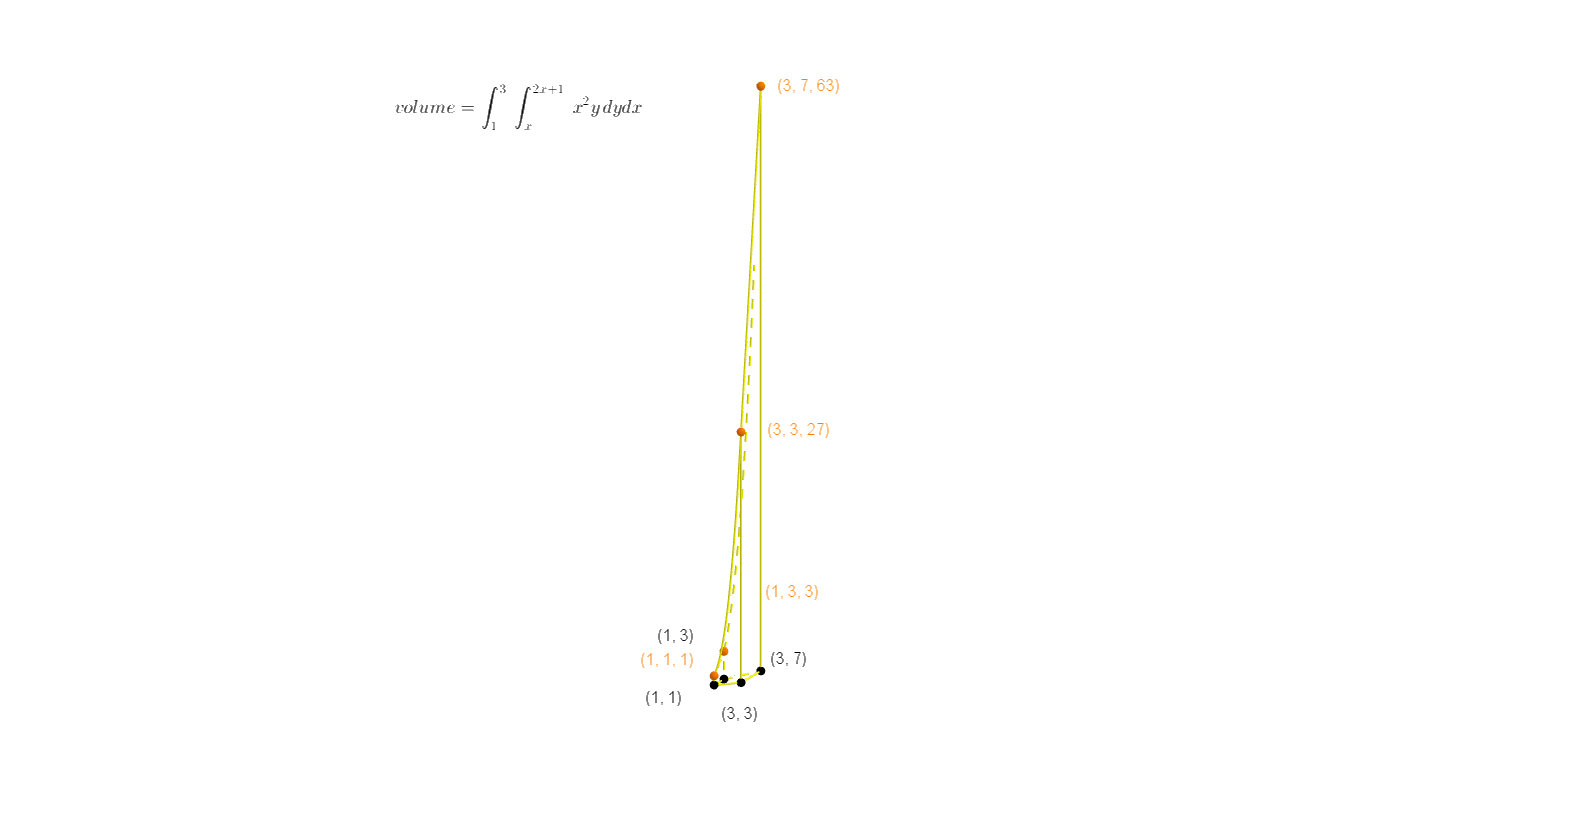
\includegraphics[width=0.5\textwidth]{v05_a05_e02.png}		
	\end{figure}
	
	\begin{gather*}
		v = \int_1^3 \int_x^{2x + 1} x^2y\, dy dx = \int_1^3 x^2\, dx \int_x^{2x + 1} y\, dy =  \int_1^3 x^2\, dx \left[\dfrac{y^2}{2}\right]_x^{2x + 1} =\\  \int_1^3 x^2\, dx \dfrac{1}{2}\left[(2x + 1)^2 - (x)^2\right] = \dfrac{1}{2}\int_1^3 x^2\, dx \left(3x^2 + 4x + 1\right) =\\ \dfrac{3}{2}\int_1^3 x^4\, dx + 2\int_1^3 x^3\, dx + \dfrac{1}{2}\int_1^3 x^2\, dx = \left[\dfrac{3}{2}\dfrac{x^5}{5} + 2\frac{x^4}{4} + \dfrac{1}{2}\dfrac{x^3}{3}\right]_1^3 = \left[\dfrac{3x^5}{10} + \dfrac{x^4}{2} + \frac{x^3}{6}\right]_1^3 =\\ \left[\dfrac{18x^5 + 30x^4 + 10x^3}{60}\right]_1^3 = \left[\dfrac{2x^3\left(9x^2 + 15x + 5\right)}{60}\right]_1^3 =\\ \dfrac{1}{30}\left[x^3\left(9x^2 + 15x + 5\right)\right]_1^3 = \dfrac{1}{30}\left[3^3\left(9\cdot3^2 + 15\cdot3 + 5\right) - 1^3\left(9\cdot1^2 + 15\cdot1 + 5\right)\right] =\\ \dfrac{1}{30}\left[27(81 + 45 + 5) - (9 + 15 + 5)\right] = \dfrac{1}{30}\left[27\cdot131 - 29\right] = \frac{3508}{30} = 116,9\overline{3}	
	\end{gather*}
\end{enumerate}